\section{Evaluation Suchalgorithmus}
Die Evaluation verschiedener Algorithmen zur Erkennung von Fussgängerstreifen stellt ein wichtiger Teil unserer Arbeit dar. Um die Kandidaten zu vergleichen griffen wir auf das Werkzeug der Confusion Matrix (Wahrheitsmatrix) zurück.

\subsection{Algorithmen Vergleich}
Um einen nachvollziehbaren Vergleich durchzuführen haben wir mit folgenden Eckdaten gearbeitet:
\begin{tabbing}[H]
    \hspace*{6cm}\=\hspace*{6cm}\= \kill
    Bounding Box (Rapperswil): \> (8.814650, 47.222553, 8.825035, 47.228935) \\
    Anzahl Fussgängerstreifen: \> 37 \\
\end{tabbing}

\subsubsection{Haar Feature-based Cascade Classifier}
\begin{figure}[H]
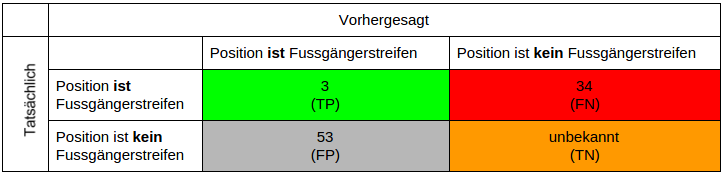
\includegraphics[width=\textwidth]{images/haar_conf.png}
\caption[Haar Feature-based Cascade Classifier]{Haar Feature-based Cascade Classifier}
\end{figure}
\subsubsection{Fast Fourier Transform}	
\begin{figure}[H]
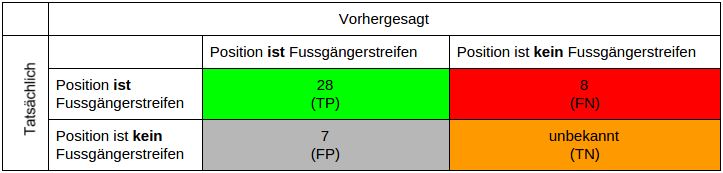
\includegraphics[width=\textwidth]{images/fast_fourier_conf.png}
\caption[Fast Fourier Transform]{Fast Fourier Transform}
\end{figure}
\subsubsection{Scale-invariant Feature Transform}	
\begin{figure}[H]
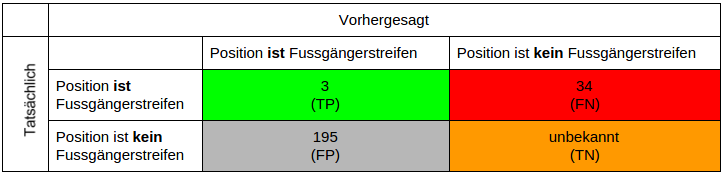
\includegraphics[width=\textwidth]{images/sif_conf.png}
\caption[Scale-invariant Feature Transform]{Scale-invariant Feature Transform}
\end{figure}
\subsubsection{Deep Learning}	
\begin{figure}[H]
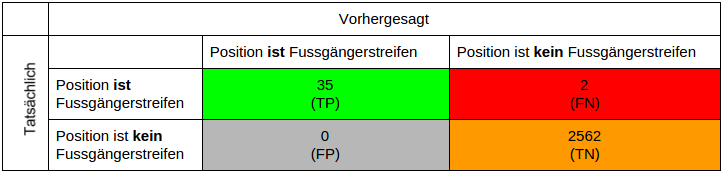
\includegraphics[width=\textwidth]{images/deep_conf.png}
\caption[Deep Learning]{Deep Learning}
\end{figure}
\subsection{Auswertung}
Damit die Auswertung verständlich ist, wird hier noch auf die Berechnung und die angeführte Legende verwiesen.
\subsubsection{Legende}
\begin{tabbing}
    \hspace*{3cm}\=\hspace*{6cm}\= \kill
    TP:	\> Zahl der richtig positiven Klassifikationen\\
	FP:	\> Zahl der falsch positiven Klassifikationen\\
	TN:	\> Zahl der richtig negativen Klassifikationen\\
	FN:	\> Zahl der falsch negativen Klassifikationen\\
\end{tabbing}

\subsubsection{Berechnung}
\begin{tabbing}
    \hspace*{3cm}\=\hspace*{3cm}\=\hspace*{6cm}\= \kill
	Trefferquote \> = \> TP / (TP+FN)\\
	Richtigkeit \> = \> (TP + TN) / (TP + FP + TN + FN)\\
	Relevanz \> = \> TP / (TP + FP)\\
\end{tabbing}

\begin{table}[H]
    \begin{tabular}{|l|l|l|l|}
    \hline    
    \rowcolor{lightblue}
	Algorithmus & Tefferquote & Richtigkeit & Relevanz \\ \hline
	Haar Feature-based Cascade Classifier & 0.08 & 0.97 & 0.05 \\ \hline
	Scale-invariant feature transform & 0.08 & 0.91 & 0.02 \\ \hline
	Fast Fourier Transform & 0.77 & 0.99 & 0.8 \\ \hline
	Deep learning & 0.95 & 0.99 & 1.0 \\ \hline
    \end{tabular}
    \caption[Algorithmen Vergleich]{Algorithmen Vergleich}
\end{table}

\decision{Evaluation Suchalgorithmus}
An dieser stelle ist zu erwähnen, dass Bilderkennung im Allgemeinen ein nicht triviales Problem ist. Man hat mit den unterschiedlichsten Schwierigkeiten zu kämpfen, wie der qualität oder die Belichtung der Bilder. Das führte dazu, dass nur mit dem Fast Fourier Transform und dem Deep Learning Ansatz Resultate erziehlt wurden, welche ein brauchbares Ergebnis lieferten. Der Deep Learning ist jedoch der klare Favoirt und sticht insbesondere beim Fals Positive Wert hervor. Deshalb entschieden wir uns, unser Fokus auf diesen Algorithmus zu legen. 



